\section{Domain Model}
\label{sec:domain_model}

\subsection{Domain Model Diagram}
\label{subsec:domain_model_diagram}
\begin{figure}[H]
    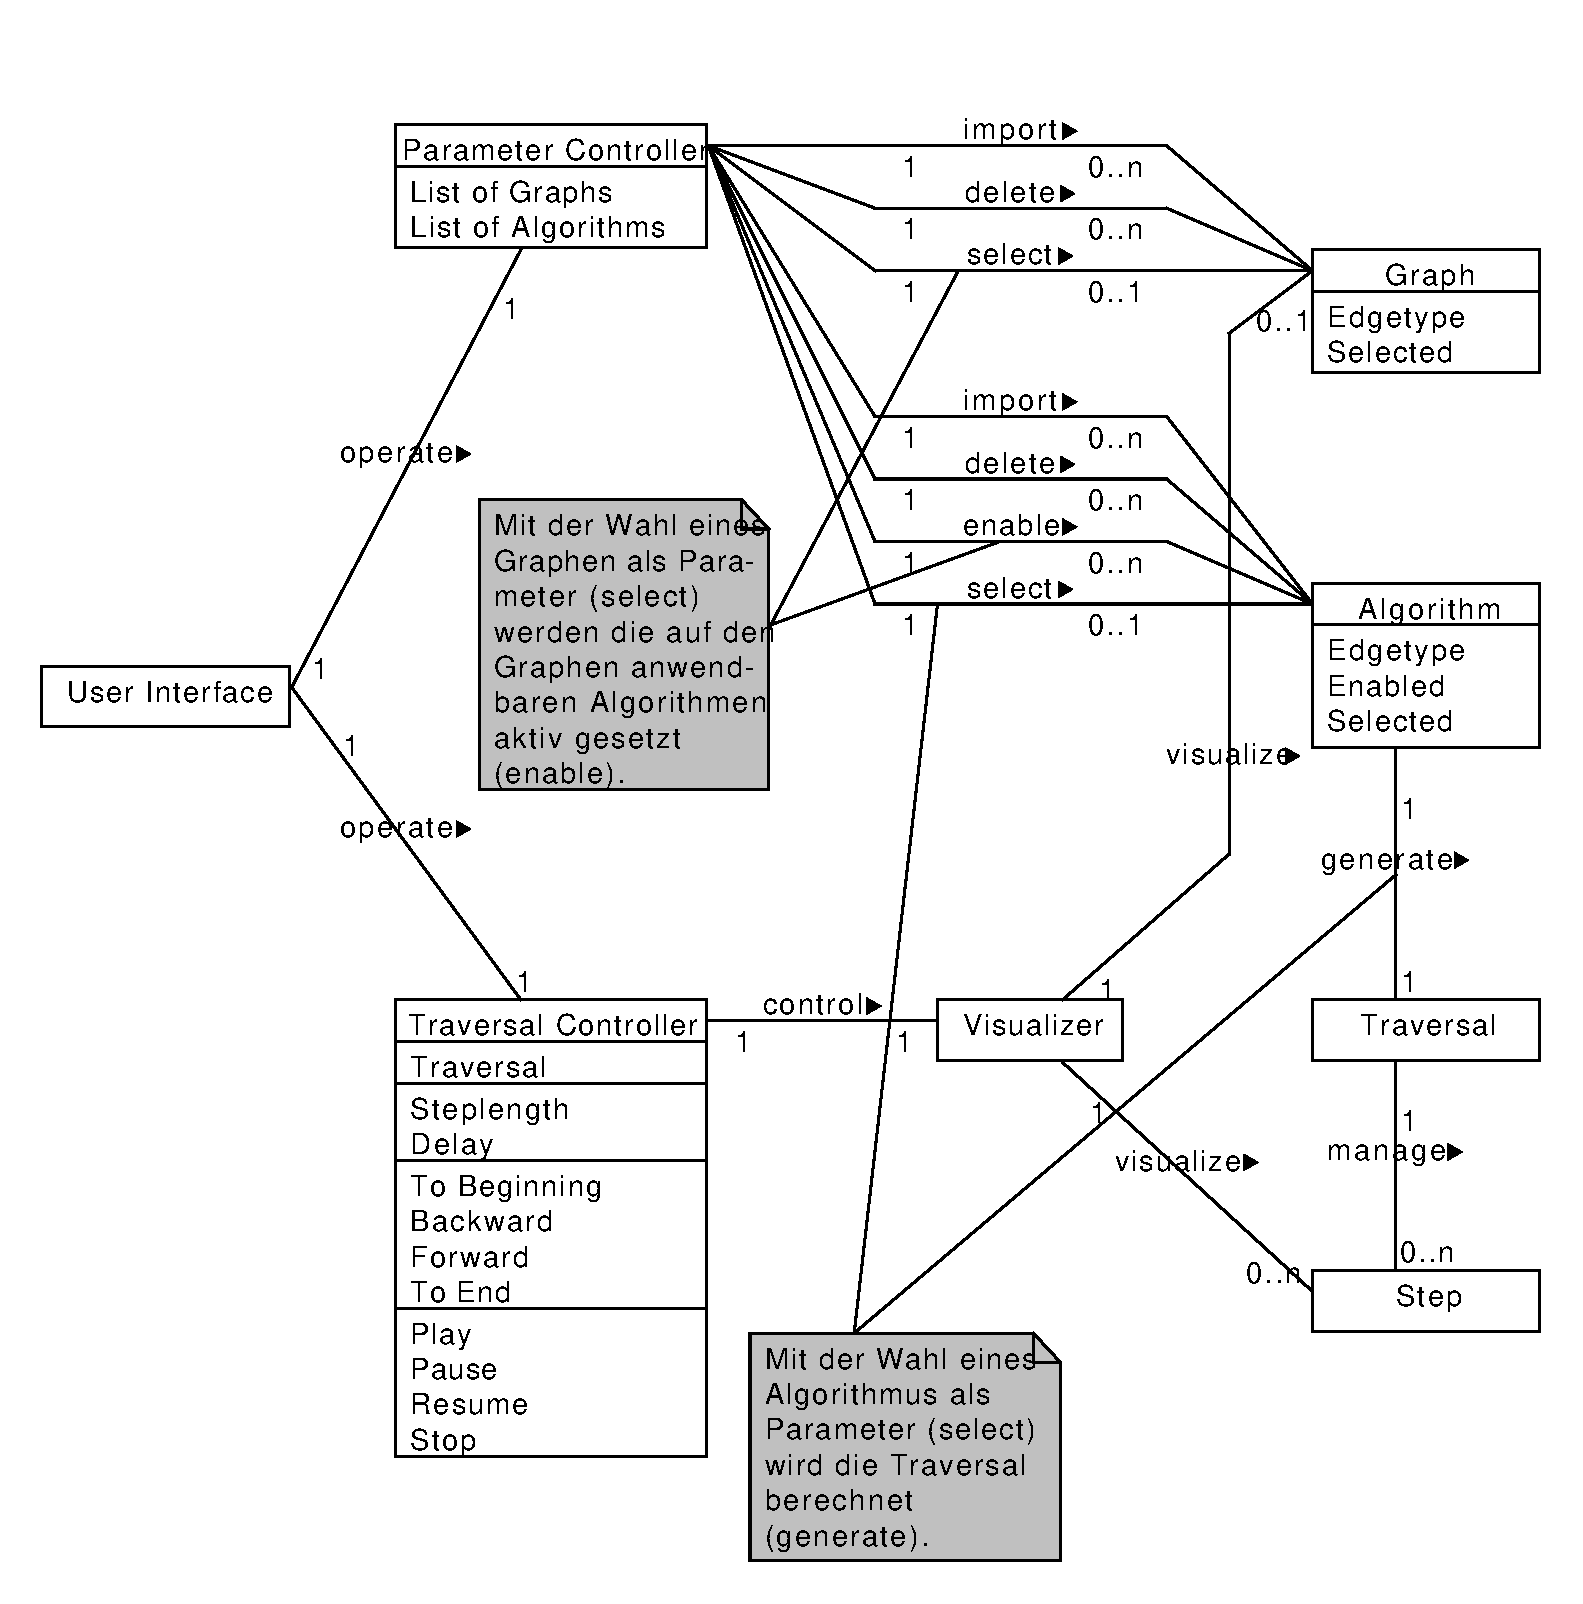
\includegraphics[totalheight=0.55\textheight]{diagrams/domain-model-diagram.pdf}
    \caption{Domain Model Diagram}
    \label{fig:domain_model_diagram}
\end{figure}

\newpage
\subsection{Domain Model Description}
\label{subsec:domain_model_description}
Es folgt eine Beschreibung der Konzeptklassen (conceptual class) mit Assoziationen, wie im Domain Model Diagram gezeigt. Attribute und Multiplizit\"aten werden in Klammern angegeben.

\subsubsection{User interface}
\label{subsubsec:User interface}
\begin{itemize}
  \item \"Uber ein User Interface (1) kann ein User einen Traversal Manager (1) bedienen (\textit{operate}).
  \item \"Uber ein User Interface (1) kann ein User einen Traversal Player (1) bedienen (\textit{operate}).
\end{itemize}
% 
\subsubsection{Traversal Manager}
\label{subsubsec:Traversal Manager}
\begin{itemize}
  \item Ein Traversal Manager h\"alt eine gegebene Anzahl Graphen als Vorlagen (\textit{List of Graphs}) bereit.
  \item \"Uber einen Parameter Manager (1) kann ein User einen oder mehrere Graphen (0..n) des Formates *.graphml importieren (\textit{import}). Diese werden der Liste mit Graphen (\textit{List of Graphs}) hinzugef\"ugt.
  \item \"Uber einen Parameter Manager (1) kann ein User vormals importierte Graphn (0..n) wieder l\"oschen (\textit{delete}). Diese werden aus der Liste mit Graphen (\textit{List of Graphs}) wieder entfernt.
  \item \"Uber einen Parameter Manager (1) kann ein User einen Graphen (1) als Parameter ausw\"ahlen (\textit{select}).
  \item Mit der Wahl eines Graphen (1) als Parameter werden die auf den Graphen anwendbaren Algorithmen (0..n) aktiv gesetzt (\textit{enable}).
  \item Ein Traversal Manager h\"alt eine gegebene Anzahl Algorithmen als Vorlagen (\textit{List of Algorithms}) bereit. Diese werden der Liste mit Algorithmen (\textit{List of Algorithms}) hinzugef\"ugt.
  \item \"Uber einen Parameter Manager (1) kann ein User einen oder mehrere Algorithmen (0..n) importieren (\textit{import}), sofern dieser die geforderten Interfaces implementiert.
  \item \"Uber einen Parameter Manager (1) kann ein User vormals importierte Algorithmen (0..n) wieder l\"oschen (\textit{delete}). Diese werden aus der Liste mit Algorithmen (\textit{List of Algorithms}) wieder entfernt.
  \item \"Uber einen Parameter Manager (1) kann ein User einen Algorithmus (1) als Parameter ausw\"ahlen (\textit{select}).
  \item Mit der Wahl eines Algorithmus (1) als Parameter wird eine Traversal (1) erstellt (\textit{generate}).
\end{itemize}
% 
\subsubsection{Graph}
\label{subsubsec:Graph}
\begin{itemize}
  \item Ein Graph hat ungerichtete oder gerichtete Kanten (\textit{Edgetype}).
  \item Ein Graph kann ausgew\"ahlt werden (\textit{Selected}).
\end{itemize}
% 
\subsubsection{Algorithm}
\label{subsubsec:Algorithm}
\begin{itemize}
  \item Ein Algorithm kann Graphen mit ungerichteten oder gerichteten Kanten (\textit{Edgetype}) verarbeiten.
  \item Ein Algorithm kann aktiviert werden (\textit{Enabled}).
  \item Ein Algorithm kann ausgew\"ahlt werden (\textit{Selected}).
  \item Ein Algorithm (1) generiert eine Traversal (1).
\end{itemize}
% 
\subsubsection{Traversal}
\label{subsubsec:Traversal}
\begin{itemize}
  \item Eine Traversal (1) kann einen oder mehrere Steps (0..n) auflisten (\textit{List of Steps}).
\end{itemize}

\subsubsection{Step}
\label{subsubsec:Step}
\begin{itemize}
  \item Ein Step ist ein Schritt der Traversierung.
\end{itemize}

\subsubsection{Traversal Player}
\label{subsubsec:Traversal Player}
\begin{itemize}
  \item Ein Traversal Player (1) steuert einen Visualizer (1).
  \item Ein Traversal Player h\"alt eine Traversierung (\textit{Traversal}).
  \item \"Uber einen Traversal Player (1) kann ein User die Anzahl Schritte (\textit{Steplength}) pro Bild einstellen.
  \item \"Uber einen Traversal Player (1) kann ein User die Zeit (\textit{Delay}) zwischen zwei Bildern einstellen.
  \item \"Uber einen Traversal Player (1) kann ein User Springen-Elemente (\textit{Forward, Backward, To Beginning, To End}) f\"ur die Step-by-Step Visualisierung im Visualizer (1) bedienen.
  \item \"Uber einen Traversal Player (1) kann ein User Abspiel-Elemente (\textit{Play, Pause, Resume, Stop}) f\"ur die animierte Visualisierung im Visualizer (1) bedienen.
\end{itemize}

\subsubsection{Visualizer}
\label{subsubsec:Visualizer}
\begin{itemize}
  \item Ein Visualizer (1) visualisiert einen Graphen (1).
  \item Ein Visualizer (1) kann einen oder mehrere Steps (0..n) visualisieren.
\end{itemize}